\chapter{Intro to Neural Networks}

Now that we know the basic algorithms underpinning Neural Networks, we need to learn how to design their architectures In this lesson, we will learn how to:

\begin{itemize}
    \item Explain essential concepts in Neural Networks, including their origins
    \item Implement appropriate Neural Networks architectures
    \item Distinguish between problems based on model objectives
    \item Design Neural Networks based on the decision boundaries in the data
\end{itemize}
Taken together, these skills, combined with knowledge of backpropagation and gradient descent, give us the ability to design our Neural Networks to solve our problems.

\section{Why "Neural Networks"?}
Neural networks get their name from the fact that they are—loosely—modeled after biological neurons. Perceptrons take inputs, perform calculations on the inputs, and decide whether to return one result or another (e.g., a one or a zero).\newline

In a similar way, neurons in the brain receive inputs (such as signals from other neurons) through their branching \textit{dendrites}, and then decide whether to, in turn, send out a signal of their own.\newline

Similar to how real neurons can be connected one to another to form \textit{layers,} we will be concatenating our perceptrons—layering multiple perceptrons such that we can take the output from one and use it as the input for another.

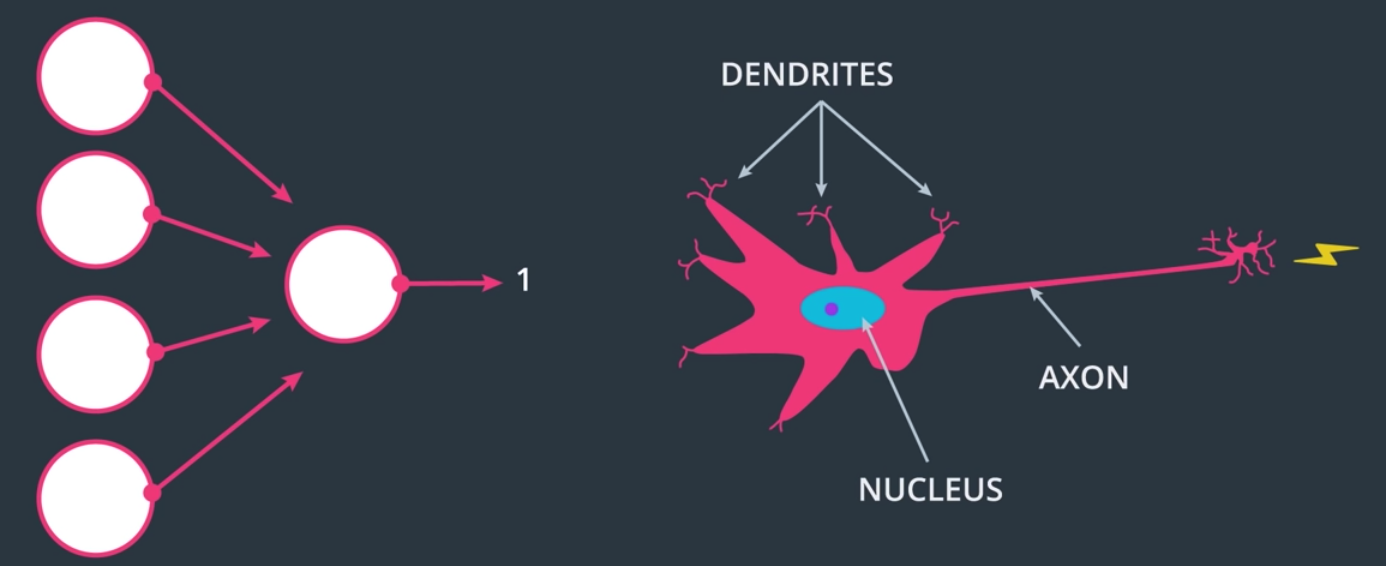
\includegraphics[width=0.75\linewidth]{img//intro/introNN/image.png}


\section{Perceptrons vs. Neural Networks}
Multilayer Perceptrons are Neural Networks. The perceptron and neural networks are inspired by biological neurons. Though modern "perceptrons" use the Logistic Sigmoid Function or other activation functions, classical perceptrons use a step function. \newline

Neural Networks are a more general class of models that encapsulates multi-layer perceptrons. Neural Networks are defined by having one or more hidden layers and an output layer that emits a decision -- either a predicted value, a probability, or a vector of probabilities, depending on the task.

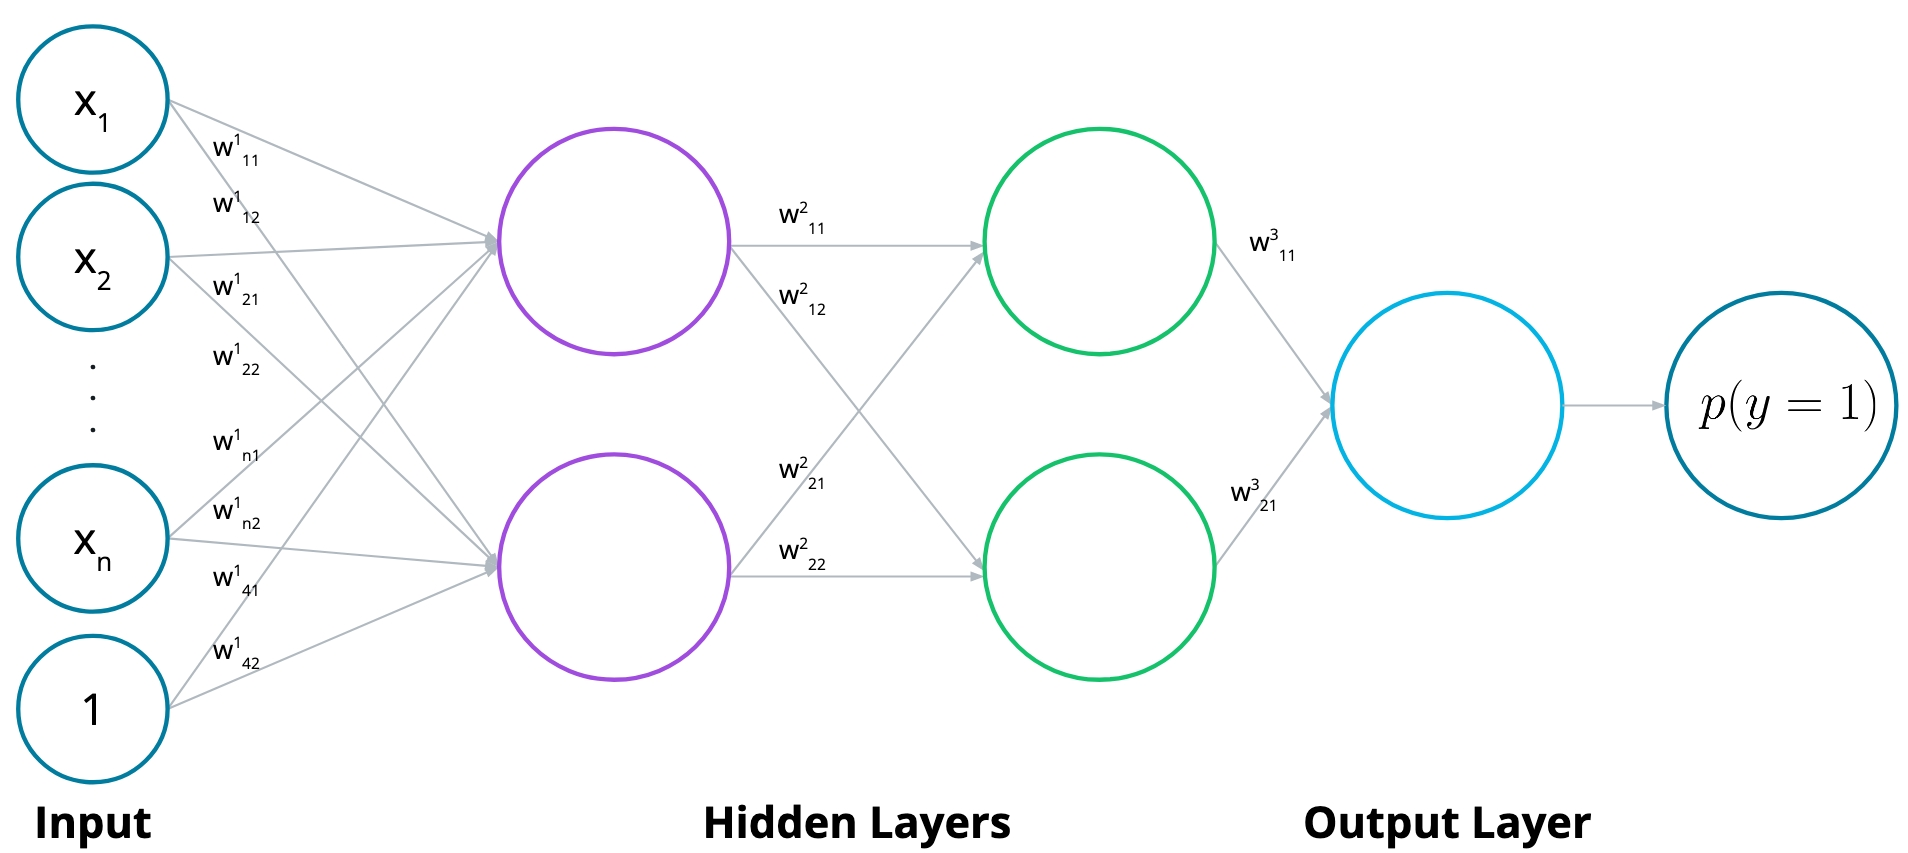
\includegraphics[width=1\linewidth]{img//intro//introNN/screen-shot-2022-05-18-at-8.52.53-am.jpeg}

\section{Neural Network Architecture}
Ok, so we're ready to put these building blocks together, and build great Neural Networks! (Or Multi-Layer Perceptrons, however you prefer to call them.) \newline

Training a model to correctly classify non-linear data like that shown above requires superimposing multiple neural networks on top of one another.

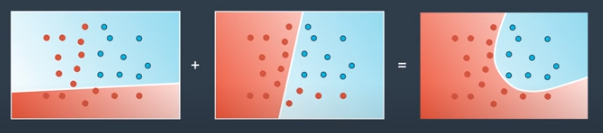
\includegraphics[width=1\linewidth]{img//intro//introNN/neural-network-architecture-2.png}

We will combine two linear models to get our non-linear model. Essentially the steps to do this are:

\begin{itemize}
    \item Calculate the probability for each model
    \item Apply weights to the probabilities
    \item Add the weighted probabilities
    \item Apply the sigmoid function to the result
\end{itemize}

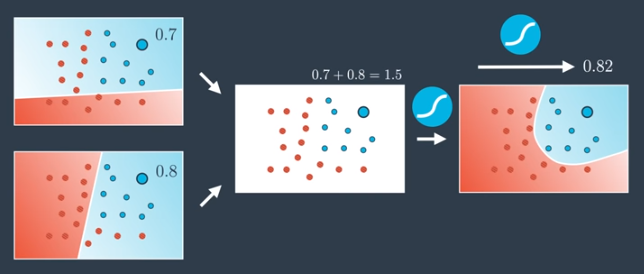
\includegraphics[width=1\linewidth]{img//intro//introNN/neural-network-architecture-3.png}

This calculation is run for every point in the plane.

\subsection{Weighting the Component Networks}
It is also possible to weight the input neural networks. For example, the model on the top left of the image below could be weighted more strongly than the model on the bottom left.

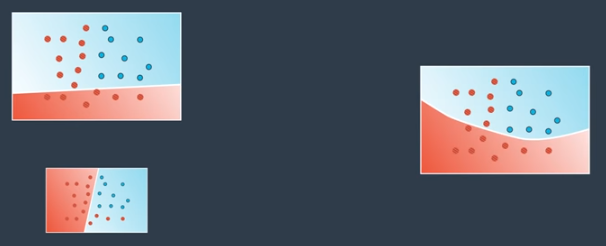
\includegraphics[width=1\linewidth]{img//intro//introNN/neural-network-architecture-4.png}

For example, the output of the top neural network could be given a weight of 7. The bottom could be given a weight of 5. An arbitrary bias of 6 could also be assigned.

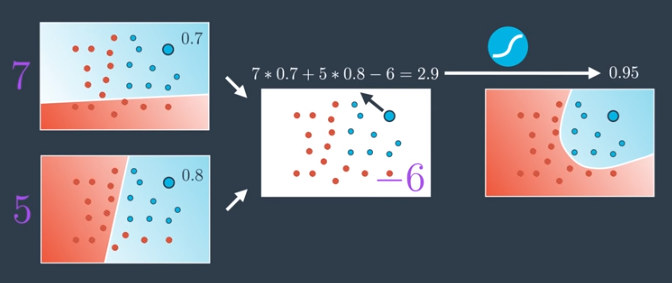
\includegraphics[width=1\linewidth]{img//intro//introNN/neural-network-architecture-5.png}

Note that this exactly how neural networks themselves operate, except instead of \textbf{inputs to a neural network} we have \textbf{neural networks, themselves}.

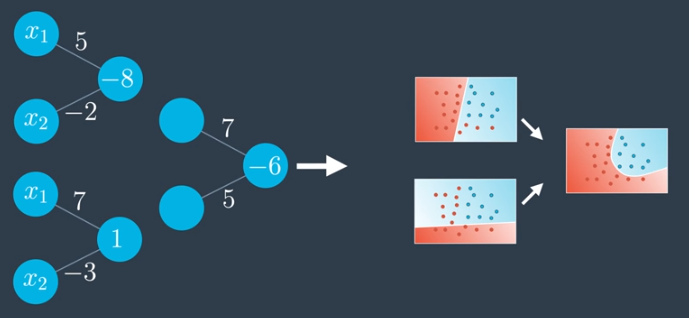
\includegraphics[width=1\linewidth]{img//intro//introNN/neural-network-architecture-6.png}

By cleaning up and consolidating the network above, we arrive at the following.

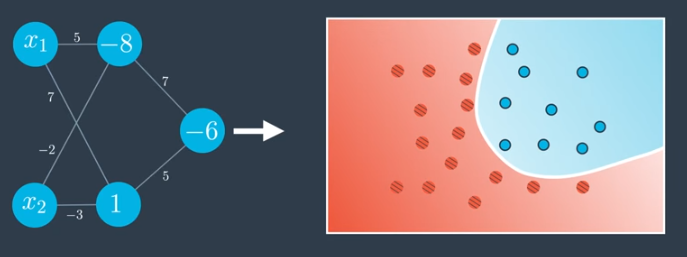
\includegraphics[width=1\linewidth]{img//intro//introNN/neural-network-architecture-7.png}

Note that the following two networks are actually identical. One uses a notation where the bias (-6) is placed inside the node. The other uses a notation where the bias comes from a single node with constant input 1 where the edges are weighted by the bias. In both cases, the sigmoid activation function is used.

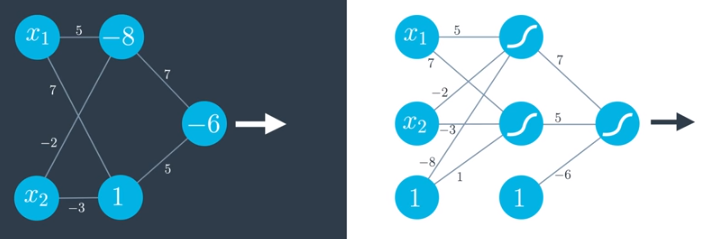
\includegraphics[width=1\linewidth]{img//intro//introNN/neural-network-architecture-8.png}

\subsection{Multiple layers}

Now, not all neural networks look like the one above. They can be way more complicated! Neural networks have a certain special architecture with layers:

\begin{itemize}
    \item The first layer is called the \textbf{input layer}, which contains the inputs.
    \item The next layer is called the \textbf{hidden layer}, which is the set of linear models created with the input layer.
    \item The final layer is called the \textbf{output layer}, which is where the linear models get combined to obtain a nonlinear model.
\end{itemize}

Neural networks can have different architectures, with varying numbers of nodes and layers:

\begin{itemize}
    \item \textbf{Input nodes.} In general, if we have \(n\) nodes in the input layer, then we are modeling data in n-dimensional space (e.g., 3 nodes in the input layer means we are modeling data in 3-dimensional space).
    \item \textbf{Output nodes.} If there are more nodes in the output layer, this simply means we have more outputs—for example, we may have a multiclass classification model.
    \item \textbf{Layers.} If there are more layers then we have a \textit{deep} neural network. Our linear models combine to create nonlinear models, which then combine to create even more nonlinear models!
\end{itemize}

\subsubsection{Adding More Nodes}
Adding more nodes to the hidden layer enables creation of more complex outputs, such as the triangular region shown below.

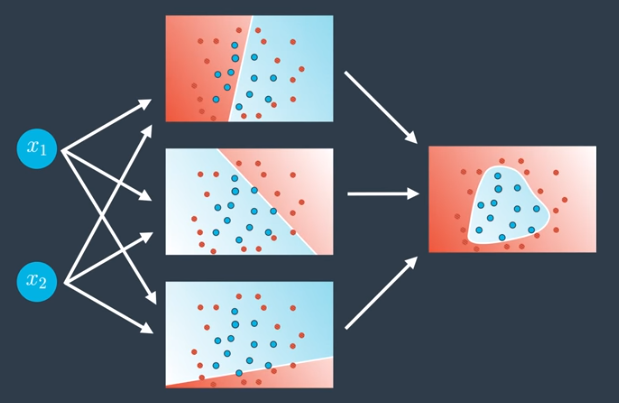
\includegraphics[width=1\linewidth]{img//intro//introNN/neural-network-architecture-10.png}

Adding more nodes to the \textbf{input layer} means the data space is higher dimensional. For example, in the network architecture below, the space is three-dimensional, the linear models in the hidden layers are planes, and the output layer bounds a nonlinear region in three space.

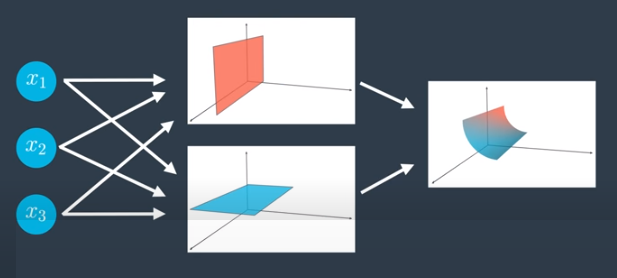
\includegraphics[width=1\linewidth]{img//intro//introNN/neural-network-architecture-11.png}

In general, if we have n dimensions in the input layer, we are living in n space. \newline

Adding more dimensions to the \textbf{output layer} means we have more outputs, and we are performing more complex, multiple-class classification.

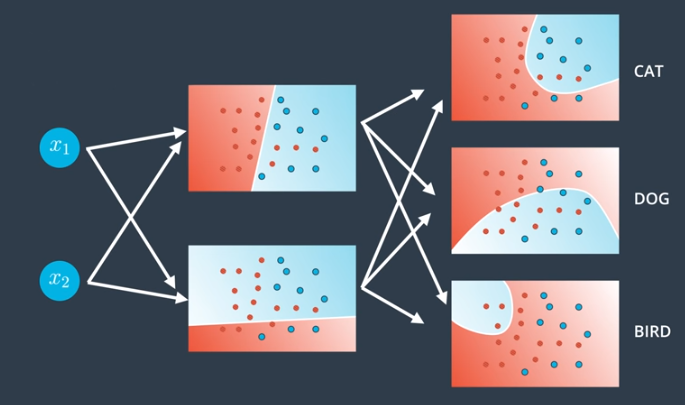
\includegraphics[width=1\linewidth]{img//intro//introNN/neural-network-architecture-12.png}

\subsubsection{Adding More Layers}

If we add more layers, we have a \textbf{deep neural network}. Our nonlinear models combine to create even more nonlinear models.

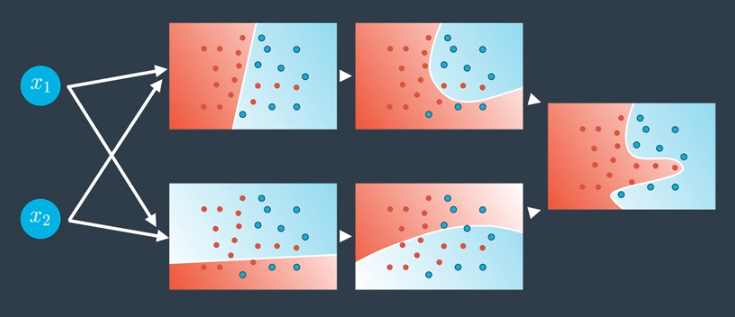
\includegraphics[width=1\linewidth]{img//intro//introNN/neural-network-architecture-13.png}

This can be done many times, creating highly complex nonlinear models. Many of the models in real life, specifically, in applications such as self-driving cars and game-playing agents, have many hidden layers.

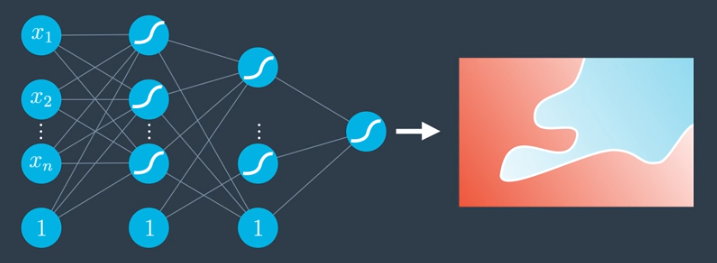
\includegraphics[width=1\linewidth]{img//intro//introNN/neural-network-architecture-14.png}

\subsection{Multi-Class Classification}
When we have three or more classes, we \textit{could} construct three separate neural networks—one for predicting each class. However, this is not necessary. Instead, we can add more nodes in the output layer. Each of these nodes will give us the probability that the item belongs to the given class.

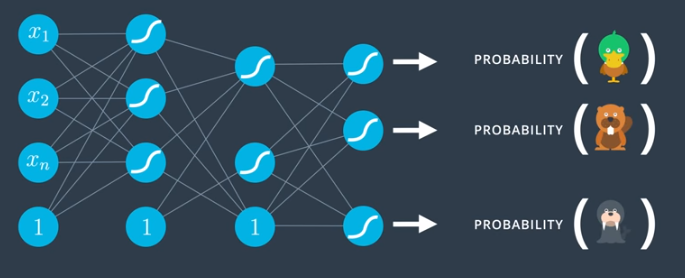
\includegraphics[width=1\linewidth]{img//intro//introNN/neural-network-architecture-15.png}

When using neural networks to perform multi-class classification, the number of outputs must match the number of classifications. Then, we use the \lstinline|softmax| function on those outputs to obtain well-defined probabilities.

\subsection{Feedforward}
\href{https://www.youtube.com/watch?v=hVCuvMGOfyY&ab_channel=Udacity}{Youtube} \newline

\textbf{Feedforward} is the process neural networks use to turn the input into an output. In general terms, the process looks like this:

\begin{itemize}
    \item Take the input vector
    \item Apply a sequence of linear models and sigmoid functions
    \item Combine maps to create a highly non-linear map
\end{itemize}
As we saw in the video, the feedforward formula is: \[\hat{y} = \sigma \circ W^{(2)} \circ \sigma \circ W^{(1)}(x)\]

\subsubsection{Feedforward in Perceptrons}
Consider the example shown in the image below. The input is given by \(x = (x_1, x_2)\), and the label is \(y = 1\).

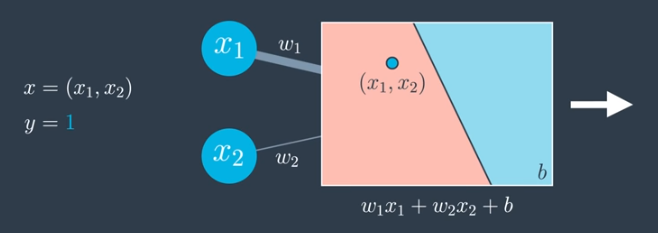
\includegraphics[width=1\linewidth]{img//intro//introNN/neural-network-architecture-16.png}

The perceptron receives the data point, \((x_1, x_2)\). The perceptron plots the point and outputs the probability that thte point is blue. Here, since the point is in the red area, the output would be a small number since the point is not very likely to be blue. But, in this case the point is blue, so the model does not appear to be very good.

\subsubsection{Feedforward in Neural Networks}
Feedforward operates in a similar manner for neural networks.

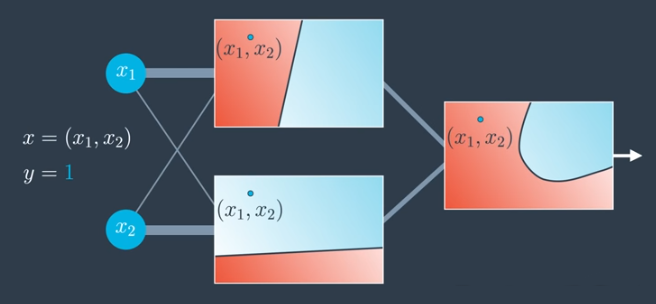
\includegraphics[width=1\linewidth]{img//intro//introNN/neural-network-architecture-17.png}

To discuss more specifically, introduce the following notation:
\begin{itemize}
    \item \(W^{(2)}\) - indicates the weight belongs to the second layer.
    \item \(W_{12}\) - indicates the weight is between the first node in the layer that is the input to the edge, and the second node in that layer that is the output to the edge.
\end{itemize}

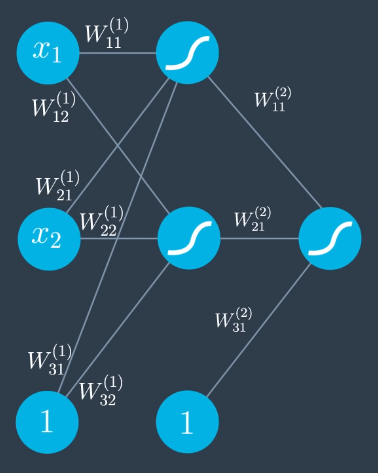
\includegraphics[width=0.75\linewidth]{img//intro//introNN/neural-network-architecture-18.png}

The output prediction, \(\hat{y}\), is given by \[\hat{y} = \sigma \Bigg( \begin{matrix}W_{11}^{(2)} \\ W_{21}^{(2)} \\ W_{31}^{(2)}  \end{matrix} \Bigg) \sigma \Bigg( \begin{matrix}W_{11}^{(1)} & W_{12}^{(1)} \\ W_{21}^{(1)} & W_{22}^{(1)} \\ W_{31}^{(1)} & W_{32}^{(1)}  \end{matrix} \Bigg) \Bigg( \begin{matrix}x_1 \\ x_2 \\ 1 \end{matrix} \Bigg)\]

A more compact representation of the same equation is shown below. \[\hat{y} = \sigma \circ W^{(2)} \circ \sigma \circ W^{(1)}(x)\]

For a 3-layer neural network, like that shown below, the equation that follows would be used.

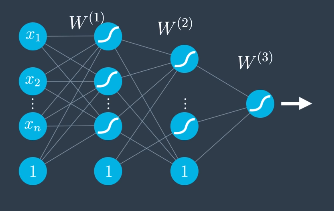
\includegraphics[width=0.75\linewidth]{img//intro//introNN/neural-network-architecture-19.png}

\[\hat{y} = \sigma \circ W^{(3)} \sigma \circ W^{(2)} \circ \sigma \circ W^{(1)}(x)\]

\subsection{Error Function}
\href{https://www.youtube.com/watch?v=SC1wEW7TtKs&ab_channel=Udacity}{Youtube} \newline

For a multilayer perceptron, as we saw, our prediction is simply a combination of matrix multiplications and sigmoid functions. But the error function can be the exact same formula, aside from the fact that \(\hat{y}\) is a bit more complicated. \[E(W) = -\frac{1}{m} \sum_{i=1}^m y_iln(\hat{y_i}) + (1-y_i) ln(1-\hat{y}_i)\]


\section{Exercise: Neural Network Architectures}

\subsubsection{Quiz Question}

Have a look at this code:
\begin{lstlisting}
class Net(nn.Module):
    def __init__(self):
        super().__init__()
        self.fc1 = Linear(1024, 128)
        self.fc2 = Linear(128, 64)
        self.fc3 = Linear(64, 1)

    def forward(self, x):
        x = relu(self.fc1(x))
        x = relu(self.fc2(x))
        x = sigmoid(self.fc3(x))
        return x
\end{lstlisting}
What does the line \verb|x = sigmoid(self.fc3(x))| do?
\begin{itemize}
    \item \textbf{Converts the output of \lstinline{self.fc3} to a probability between zero and one}
    \item Adds a layer to the neural network
    \item Computes the gradient of the input
    \item Combines the linear models in the hidden layer
\end{itemize}

\subsubsection{Quiz Question}

Assume you have the same code from question 1 above:
\begin{lstlisting}
class Net(nn.Module):
    def __init__(self):
        super().__init__()
        self.fc1 = Linear(1024, 128)
        self.fc2 = Linear(128, 64)
        self.fc3 = Linear(64, 1)

    def forward(self, x):
        x = relu(self.fc1(x))
        x = relu(self.fc2(x))
        x = sigmoid(self.fc3(x))
        return x
\end{lstlisting}
How would we modify this in a multi-class classification setting? \textit{(choose two)}
\begin{itemize}
    \item \textbf{Modify the number of output neurons in \lstinline{self.fc3}}
    \item Modify the size of the input in \lstinline{self.fc1}
    \item Change \lstinline{relu} to \lstinline{softmax}
    \item \textbf{Change \lstinline{sigmoid} to \lstinline{softmax}}
\end{itemize}


\subsubsection{Quiz Question}

Imagine you are developing a neural network that takes flattened 256 x 256 matrices as an input. Which of the following lines of code will work for your input layer?
\begin{itemize}
    \item \lstinline{self.fc1 = Linear(256, 128}
    \item \lstinline{self.fc1 = Linear(128, 256}
    \item This is the solution:\lstinline{self.fc1 = Linear(65536, 128}
    \item \lstinline{self.fc1 = Linear(128, 128}
\end{itemize}
Reasoning: Often, it's most readable to write our input layers for flattened m x n inputs as \verb|Linear(m * n, output_size)|.

\subsubsection{Quiz Question}

Imagine you are training your neural network but the accuracy is not improving -- you and your team determine that your model's decision boundary is not flexible enough to capture all the points. How could you improve your model? \textit{(Choose two)}
\begin{itemize}
    \item Increase the size of the input in the input layer
    \item \textbf{Increase the number of nodes in the hidden layers}
    \item Increase the size of  the output in the output layer
    \item \textbf{Add more layers to the model}
\end{itemize}

Reasoning: Although increasing the number of nodes in the hidden layers and adding layers to the model make it more complex, it often yields better performance.

\section{Activation Functions}
\href{https://www.youtube.com/watch?v=DhGm2clOS-U&ab_channel=Udacity}{Youtube}

\subsection{Activation Function Properties}

There are a wide variety of activation functions that we can use. Activation functions should be:

\begin{itemize}
    \item Nonlinear
    \item Differentiable, ideally continuously differentiable. That is, they have a derivative everywhere
    \item Monotonic: If you look at the function from left to right, the value on the y-axis never goes down.
    \item Close to the identity function at the origin
\end{itemize}
We can loosen these restrictions slightly. For example, ReLU is not differentiable at the origin. Others, like monotonicity, are very important and cannot be reasonably relaxed.

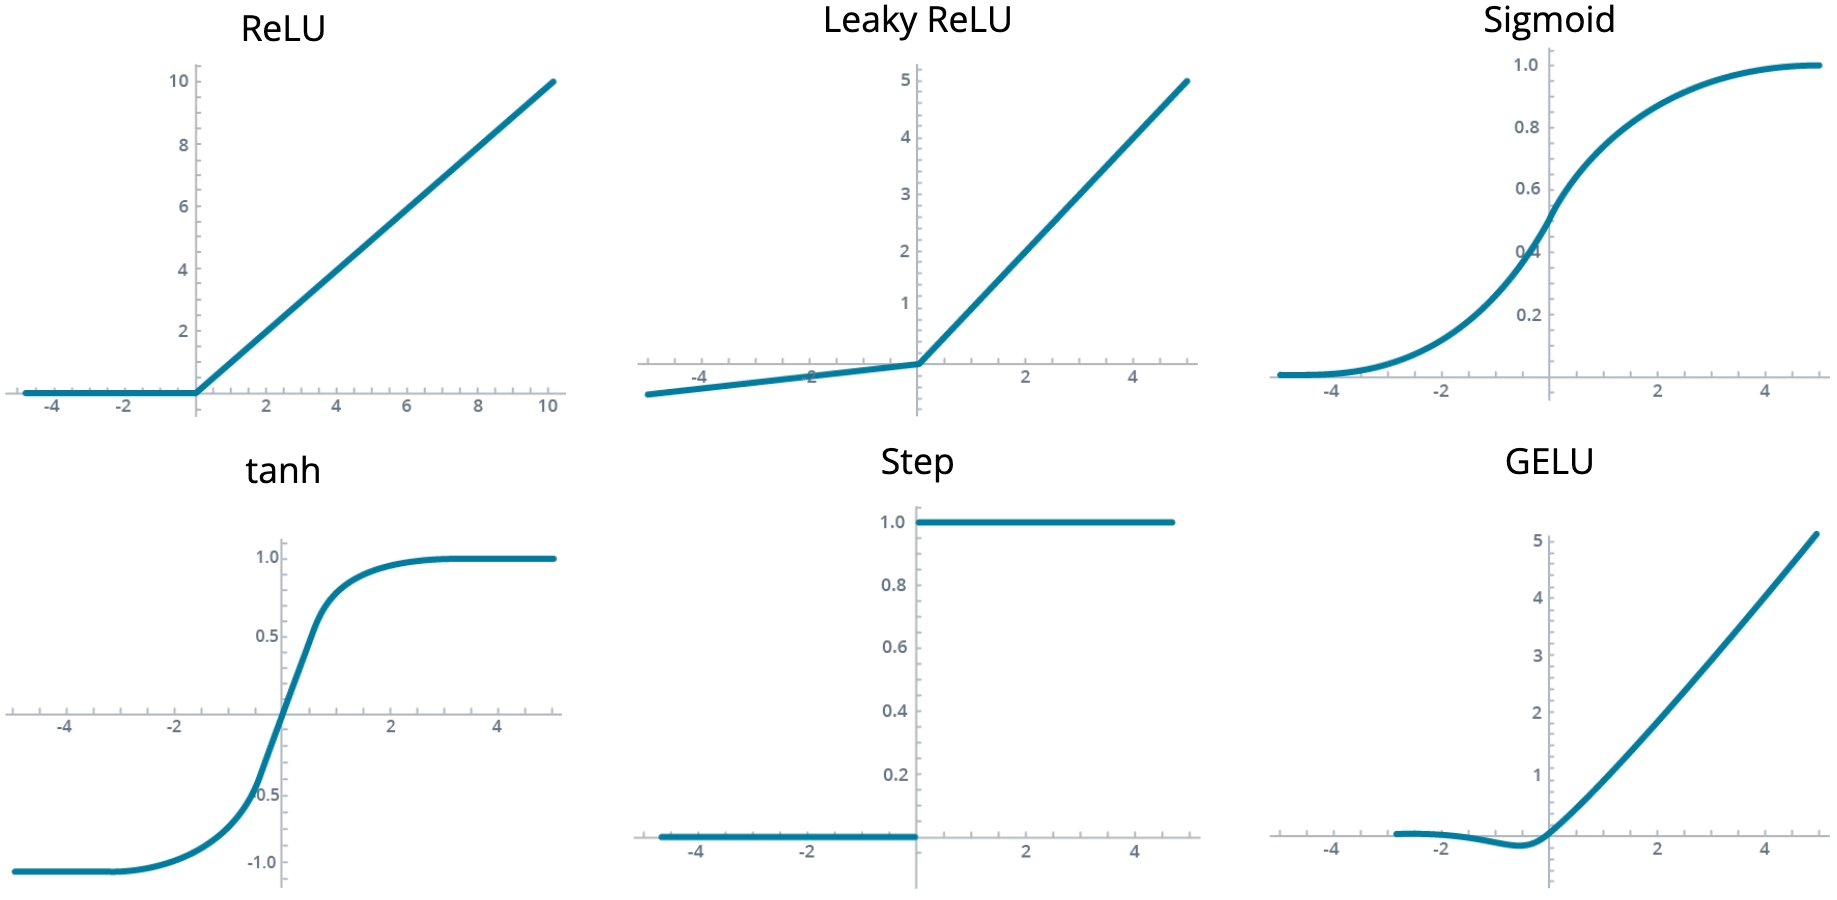
\includegraphics[width=1\linewidth]{img//intro//introNN/activation-functions.jpeg}

\paragraph{Rectified Linear Unit (ReLU)}

For many models, ReLU is the only activation function you'll see in the hidden neurons since it has great empirical performance and is easy to compute gradients on. ReLU is \textbf{not differentiable everywhere}: it is not differentiable at zero. 

\paragraph{Leaky ReLU}
Rather than zeroing out the output when it's negative, the Leaky ReLU ouputs one-tenth of the input.

\paragraph{Sigmoid}
Sigmoid bounds everything between 0 and 1. It also has easily computable derivatives. However, networks trained using sigmoid do not perform as well as those trained with ReLU. So it is rarely used in the hidden layers.

\paragraph{Hyperbolic tangent (tanh)}
Like sigmoid, tanh has the property of being bounded from above and below. Hence, all of the outputs are between -1 and +1. It is also centered at zero and has bigger derivatives than the sigmoid. 

\paragraph{Step function}

\paragraph{Gaussian Error linear units (GELU)}
GELU has been used in some transformer models, including Open AIs GPT-3.


\subsection{Quiz Question}
What factors can help you decide what activation function to use?

\textbf{Select all that apply.}

\begin{itemize}
    \item \textbf{Whether or not the activation function is bounded from above
    \item Whether or not the activation function is bounded from below
    \item The value of the activation function at the origin
    \item The ease of computing its gradient}
\end{itemize}

\section{Neural Network Objectives}
\href{https://www.youtube.com/watch?v=Q0u_THaU9n8&t=19s&ab_channel=Udacity}{Youtube} \newline

Once you know the output you're aiming for -- a binary classification, a classification into multiple classes, or a real number -- you can use that information to make decisions about your model.\newline

In particular, the combination of loss function and output activation function is dictated by the type of problem that you have.

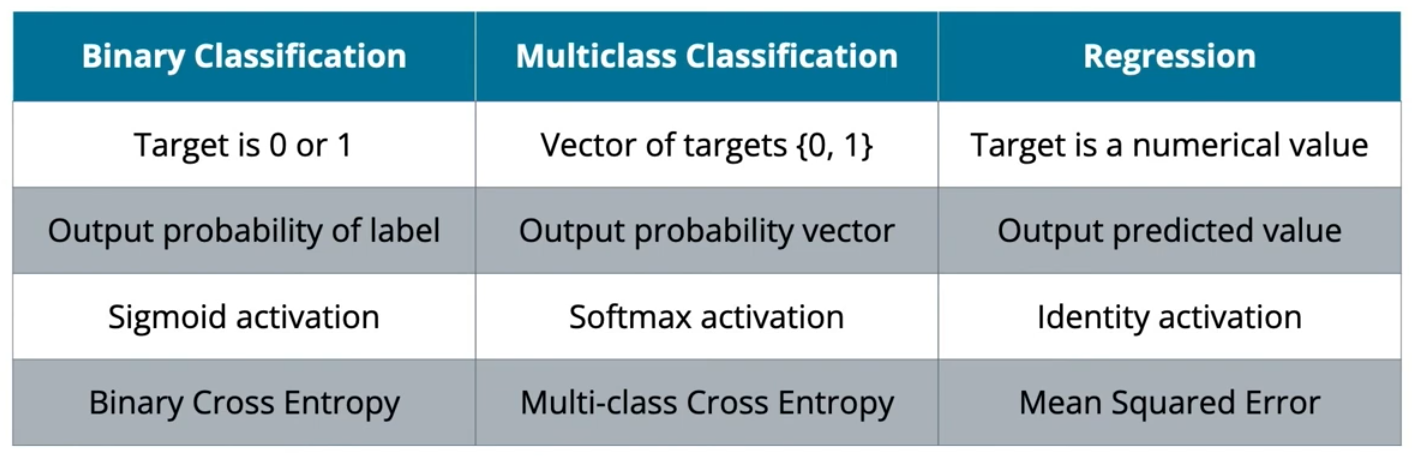
\includegraphics[width=1\linewidth]{img//intro//introNN/image2.png}

\textbf{Binary Classification:}
\begin{itemize}
    \item Target: Something that can be encoded to one or zero. E.g. whether the image is a cat or not
    \item Output layer: Sigmoid activation function
    \item Loss function we want to minimize is the binary cross-entropy
\end{itemize}

\textbf{Multiclass Classification:}
\begin{itemize}
    \item More than one class for classifiation
    \item  Target: Vector of possible targets with the length of the vector being the number of classes. The numerical value of  that class is the position in the vector. 

    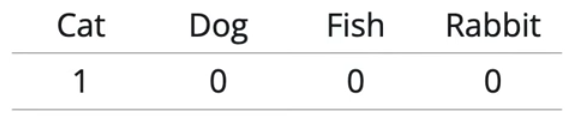
\includegraphics[width=0.5\linewidth]{img//intro//introNN/image3.png}
    
    \item The output probability vector will have values distributed across those classes. The most probable class will be the one with the highest probability.
\end{itemize}

\textbf{Regression:}
\begin{itemize}
    \item Activation function: Identity or bounded (so we do not get negative values with something like ReLU)
    \item Error functions: Mean Squared Error or Mean Absolute Error
\end{itemize}

\section{Decision Boundaries}
\href{https://www.youtube.com/watch?v=aPgH8Ra30T0&ab_channel=Udacity}{Youtube} \newline

Our data will dictate what the shape of our decision boundary should be. Neural networks will be able to find decision boundaries that are high-dimensional and nonlinear by combining the decision boundaries of the hidden neurons. Even in cases where we cannot visualize our decision boundary easily, knowing the approximate complexity of our decision boundary will inform how big our model needs to be. 

\subsection{Linear Decision Boundaries}
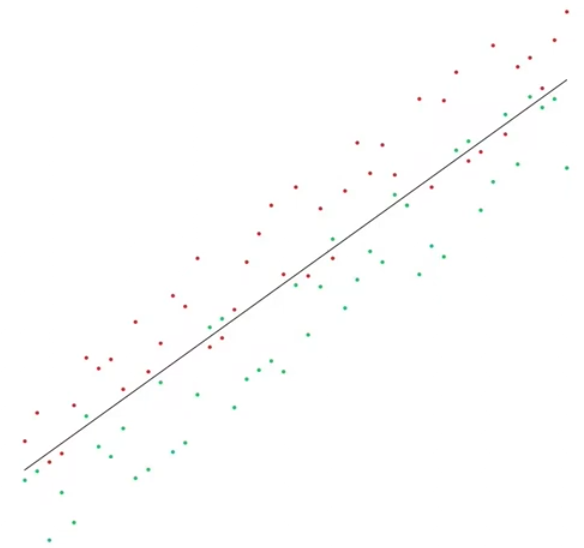
\includegraphics[width=0.25\linewidth]{img//intro//introNN/image4.png}
\begin{itemize}
    \item simplest kinds of decision bounds
    \item Straight line that best divides the data
    \item Binary classes and two dimensions
    \item Rarely want to use neural networks
\end{itemize}

\subsection{Higher Dimensional Decision Boundaries}
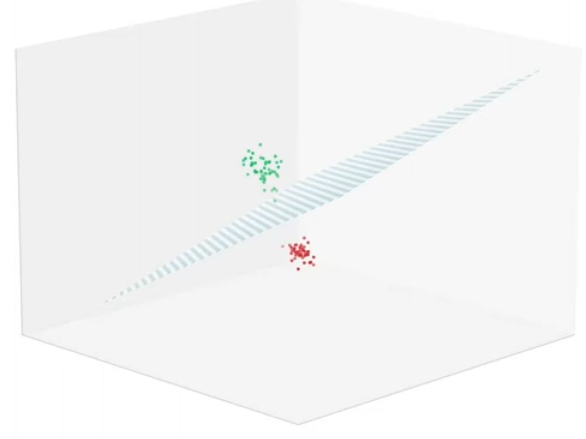
\includegraphics[width=0.25\linewidth]{img//intro//introNN/image5.png}
\begin{itemize}
    \item Divide classes with a hyperplane
    \item Given \(n\) variables, output \(n - 1\) dimensional hyperplane
    \item Cannot visualize hyperplanes in dimension greater than 3
    \item Still linear and not common for neural networks
\end{itemize}

\subsection{Nonlinear Decision Boundaries}
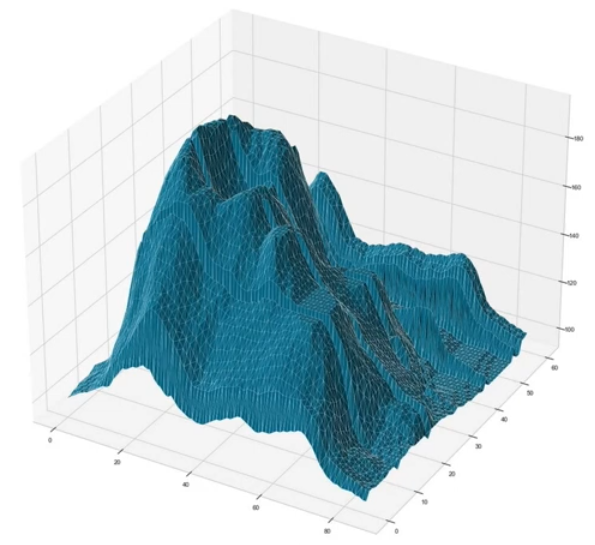
\includegraphics[width=0.25\linewidth]{img//intro//introNN/image6.png}
\begin{itemize}
    \item High-dimensional, non-linear hyperplanes are common in neural networks
    \item Since each neuron is introducing some hyperplane and we are aggregating the hyperplanes of these various neurons, these hyperplanes can be 100+ dimensions
    \item Nearly impossible to visualize decision boundaries. Can sometimes try to visualize with t-SNE
    \item Complex data = complex decision boundary
    \item Complex decision boundary = big neural network
\end{itemize}


\section{Quiz Question}

Look at the following code snippet, an example of the classic \href{https://en.wikipedia.org/wiki/LeNet}{\textbf{LeNet-5}} model:
\begin{lstlisting}
class Net(nn.Module):
    def __init__(self):
        super().__init__()
        self.conv1 = nn.Conv2d(3, 6, 5)
        self.pool = nn.MaxPool2d(2, 2)
        self.conv2 = nn.Conv2d(6, 16, 5)
        self.fc1 = nn.Linear(16  *5*  5, 120)
        self.fc2 = nn.Linear(120, 84)
        self.fc3 = nn.Linear(84, 10)

    def forward(self, x):
        x = self.pool(F.relu(self.conv1(x)))
        x = self.pool(F.relu(self.conv2(x)))
        x = torch.flatten(x, 1) 
        x = F.relu(self.fc1(x))
        x = F.relu(self.fc2(x))
        x = self.fc3(x)
        return x
\end{lstlisting}
How would you need to modify it for the road hazard detection system, assuming we are using \href{https://pytorch.org/docs/stable/generated/torch.nn.BCELoss.html\#torch.nn.BCELoss}{\textbf{\lstinline{nn.BCELoss}}} as our loss function?

(Select all that apply.)
\begin{itemize}
    \item Add more hidden layers
    \item \textbf{Change the size of the output layer}
    \item \textbf{Add an activation function to the output layer}
    \item Change the \lstinline{Linear} layers to \lstinline{Conv2d} layers
\end{itemize}

Answer: The output layer should have a single sigmoid-activated neuron that gives us a probability that there is a hazard in the road.


\section{Glossary}

For your reference, here are all the new terms we introduced in this lesson:

\begin{itemize}
    \item \textbf{Neural Networks} are defined by having one or more hidden layers and an output layer that emits a decision -- either a predicted value, a probability, or a vector of probabilities, depending on the task.
    \item \textbf{Neural Networks Layers:}

\begin{itemize}
        \item The first layer is called the \textbf{input layer}, which contains the inputs.
        \item The next layer is called the \textbf{hidden layer}, which is the set of linear models created with the input layer.
        \item The final layer is called the \textbf{output layer}, which is where the linear models get combined to obtain a nonlinear model.
\end{itemize}

    \item \textbf{Neural Network Nodes:}

\begin{itemize}
        \item \textbf{Input nodes.} In general, if we have\textit{n} nodes in the input layer, then we are modeling data in n-dimensional space (e.g., 3 nodes in the input layer means we are modeling data in 3-dimensional space).
        \item \textbf{Output nodes.} If there are more nodes in the output layer, this simply means we have more outputs—for example, we may have a multiclass classification model.
        \item \textbf{Layers.} If there are more layers then we have a \textit{deep} neural network. Our linear models combine to create nonlinear models, which then combine to create even more nonlinear models!
\end{itemize}

    \item \textbf{Feedforward} is the process neural networks use to turn the input into an output.
\end{itemize}
